%! Author = manuel
%! Date = 03.05.21

% compile with pdflatex ./'Report.tex'

% Requirements for this document:

% The submission includes a file in the root of the GitHub repository or zip file (one of Report.md, Report.ipynb, or Report.pdf) that provides a description of the implementation
% The report clearly describes the learning algorithm, along with the chosen hyperparameters. It also describes the model architectures for any neural networks.
% A plot of rewards per episode is included to illustrate that the agent is able to receive an average reward (over 100 episodes) of at least +13. The submission reports the number of episodes needed to solve the environment.
% The submission has concrete future ideas for improving the agent's performance

% Preamble
\documentclass[12pt,a4paper]{article}

% Packages
\usepackage{amsmath}
\usepackage{float}
\usepackage[hscale=0.8,vscale=0.8]{geometry}
\usepackage{amsfonts}
\usepackage{graphicx}

% Document
\begin{document}

    \section{Overview}\label{sec:overview}
    The goal of this project is to train an agent with a double-jointed arm to follow a sphere.
    The agent receives a reward of +0.1 in every step where the hand of the agent is inside the sphere.
    This example can be easily transferred to the real world, where it is a common challenge to program a robot arm to reach a certain point in space.
    \\
    For training the agent I used a DDPG (Deep Deterministic Policy Gradient) algorithm.
    DDPG was chosen over Q learning because it performs way better in a problem with continuous action spaces.
    Nevertheless, this Project uses multiple ideas from Q learning in addition to the DDPG algorithm:
    \\\\
    \textbf{Replay memory:}\\
    The agent utilizes the experience replay technique during training.
    It stores each experience in a buffer.
    In the learning step the agent will query a random sample from the buffer and learns from those randomly sampled experiences.
    \\\\
    \textbf{Target networks:}\\
    When updating the weights of the neural network of the agent we not only update the value for $Q(s,a)$ but also of other state action pairs $Q(s',a')$.
    This can lead to a very unstable training of the agent.
    In order to stabilize the training we use two neural networks: \\
    The \textbf{local network} is trained at every step to get the best prediction for the Q-value.\\
    The agent uses the \textbf{target network} to choose actions.
    In this project the target network is updated by Soft Update from the local network.
    \\\\
    Additionally the DDPG algorithm introduces the actor/critic technique.
    The critic receives a state, and an action as input and estimates the expected reward for this state, action tuple.
    The actor receives a state and outputs an action vector with each value corresponding to a continous action.
    \\\\
    The state space consists of 33 continuous states from which the agent estimates 4 continous action values.
    Both networks (actor \& critic) consist of three fully connected layers with a node size of 128 for the first and second layer.
    However, the Actor network uses a tanh activation function for the last layer to get a value between -1 and 1.


    \section{Results}\label{sec:results}
    After training for 303 episodes I was able to achieve a mean score of 30 over 100 consecutive episodes.
    Figure 1 shows the scores received in the different episodes.

    \begin{figure}[H]
        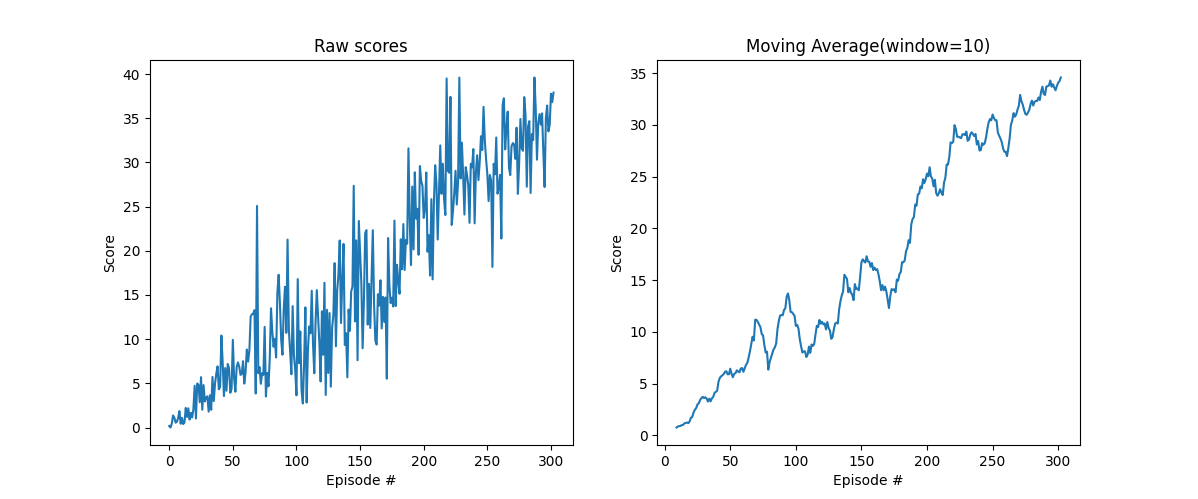
\includegraphics[width=\linewidth]{img/scores}
        \caption{Scores that the agent achieved per episode}
        \label{fig:scores}
    \end{figure}

    I achieved these scores using the following \textbf{hyper parameters}:
    \begin{center}
        \begin{tabular}{||l c l||}
            \hline
            Parameter    & Value      & Description \\ [0.5ex]
            \hline\hline
            gamma        & 0.99       & discount factor                                                           \\
            \hline
            lr\_actor    & 0.0002     & learning rate of the actor network                                        \\
            \hline
            lr\_critic   & 0.0003     & learning rate of the critic network                                       \\
            \hline
            tau          & 0.002      & update factor for soft update                                             \\
            \hline
            buffer\_size & $1*10^{6}$ & Size of the experience replay buffer                                      \\
            \hline
            batch\_size  & 128        & minibatch size (how many samples are drawn from the buffer when learning) \\
            \hline
        \end{tabular}
    \end{center}


    \section{Ideas for future improvements}\label{sec:ideas}
    Parallelize the training to multiple agents at the same time.
    This could for example be implemented with the advantage actor critic (A2C) Algorithm where multiple agents share the same network.

    \pagebreak


    \section{Useful Formulas}\label{sec:formulars}
    \textbf{Update rule for actor:}
    $$\nabla_{\theta^{\mu}}J\approx \mathbb{E}_{s_{t}\sim p^{\beta}}[\nabla_{\theta^{\mu}}Q(s,a|\theta^{Q})|s=s_{t}, a=\mu(s_{t}|\theta^{\mu})]$$
    The gradient ($\nabla$) of the cost function $J$ with respect to the network parameters $\theta$ of our actor network (denoted by $\mu$).
    \\\\
    \textbf{Update rule for critic:}
    $$L=\frac{1}{n}\sum_{i}{(y_{i}-Q(s_{i}, a_{i}|\theta^{Q}))^{2}}$$
    The critic is trying to minimize this loss function.
    \\\\
    \textbf{Soft Update:}
    $$\theta^{Q'}\leftarrow \tau\theta^{Q}+(1-\tau)+\theta^{Q'}$$
    $$\theta^{\mu'}\leftarrow \tau\theta^{\mu}+(1-\tau)+\theta^{\mu'}$$
    Where $\theta^{Q}$ are the weights of the local critic network and $\theta^{\mu}$ is the local actor network

\end{document}